% !TeX program = lualatex

\documentclass[11pt,a4paper,twocolumn]{article}

% ============================================================
% PAGE SETUP
% ============================================================

\usepackage[
    a4paper,
    top=2cm,
    bottom=2cm,
    left=2cm,
    right=2cm
]{geometry}

% ============================================================
% FONT
% ============================================================

\usepackage{fontspec}

% Assignment requires Cambria.
% Explicitly define all Cambria font styles.
\IfFontExistsTF{Cambria}{
    \setmainfont{Cambria}[
        BoldFont       = {Cambria Bold},
        ItalicFont     = {Cambria Italic},
        BoldItalicFont = {Cambria Bold Italic}
    ]
}{
    % Fallback only if Cambria is unavailable
    \setmainfont{TeX Gyre Termes}
}

% ============================================================
% LINE SPACING
% ============================================================

\usepackage{setspace}
\setstretch{1.15}

% ============================================================
% MATHEMATICS
% ============================================================

\usepackage{amsmath}
\usepackage{amssymb}

% ============================================================
% FIGURES AND TABLES
% ============================================================

\usepackage{graphicx}
\usepackage{booktabs}
\usepackage{caption}

% Approx. 10 pt italic captions
\captionsetup{
    font={small,it},
    labelfont={bf,it}
}

% ============================================================
% REFERENCES
% ============================================================

\usepackage{cite}

% ============================================================
% SECTION FORMATTING
% ============================================================

\usepackage{titlesec}

% Roman numerals: I, II, III...
\renewcommand{\thesection}{\Roman{section}}

% Section headings:
% 12 pt, bold, left aligned
\titleformat{\section}
    {\fontsize{12}{14}\selectfont\bfseries}
    {\thesection.}
    {0.5em}
    {}

\titlespacing*{\section}
    {0pt}
    {8pt}
    {4pt}

% ============================================================
% PAGE NUMBERS
% ============================================================

\pagestyle{plain}

% ============================================================
% GENERAL SPACING
% ============================================================

\setlength{\columnsep}{0.6cm}
\setlength{\parindent}{1em}
\setlength{\parskip}{0pt}

\raggedbottom


% ============================================================
% DOCUMENT
% ============================================================

\begin{document}


% ============================================================
% TITLE AND AUTHORS
% ============================================================

\twocolumn[
\begin{@twocolumnfalse}

\begin{center}

{\fontsize{14}{17}\selectfont\bfseries
Analysis of Deep Learning Architectures for
Real-Time Facial Recognition
\par}

\vspace{0.4cm}

{\fontsize{11}{13}\selectfont
Rahul Banyala (KU2407U434) \\
Prachi Ranjan (KU2407U433) \\
Rishu Pandey (KU2407U436) \\
Gauri Mahesh Adelkar (KU2407U401)
\par}

\end{center}

\vspace{0.3cm}

\end{@twocolumnfalse}
]


% ============================================================
% ABSTRACT
% Required: 120--200 words
% ============================================================

\begin{abstract}

This study deals with the real-time recognition of people using CNN-based deep learning models. It reviews and compares four different architectures: LightCNN-9, FaceNet, [Architecture 3], and [Architecture 4]. The comparison uses the experimental results and figures reported in the original research papers. Wherever possible, results obtained using the same facial dataset and evaluation protocol are selected to maintain a fair comparison. The models are compared based on recognition accuracy, computational requirements, inference speed, and suitability for real-time use. The study aims to identify which architecture provides the best balance between recognition performance and computational efficiency for a real-time facial recognition system. Later, the best-performing model will be used to build a real-time face recognition system using our own dataset.

\end{abstract}


% ============================================================
% I. INTRODUCTION
% Required: approximately 800 words
% ============================================================

\section{Introduction}

Facial recognition is a domain of computer vision that deals with recognising a human face and assigning a label or identity to it. It is commonly used in security systems, access control, attendance monitoring, surveillance, mobile-device authentication, and the organisation of digital images. Unlike face detection, which only finds the location of a face within an image, facial recognition attempts to determine the identity of the detected person. In a real-time facial recognition system, this complete process must be performed quickly enough to recognise people from a live image or video stream. Therefore, such a system requires not only good recognition accuracy but also efficient processing and a suitable response time.

The major challenge in facial recognition lies in the large variety of human faces and the different conditions in which facial images can be captured. Changes in the surrounding environment, lighting, facial position, camera angle, facial expression, and distance from the camera can significantly affect recognition performance. Other factors, such as low image resolution, image size, partial facial obstruction, background variation, ageing, and poor camera quality, can make the task even more difficult. The same person may appear different under different conditions, while two different people may sometimes have similar facial features. A reliable facial recognition model must therefore learn the important features that represent a person's identity while reducing the effect of these unwanted variations.

Within this field, Convolutional Neural Networks (CNNs) have become one of the major deep learning models used for recognising and classifying images. CNNs learn features directly from image data through hierarchical representations. The earlier layers generally learn simple features such as edges, lines, and textures, while the deeper layers learn more complex patterns such as facial structures and identity-related features. Their local connectivity and shared-weight mechanism allow them to process images efficiently and make them highly versatile for different image-related tasks. However, different CNN architectures may produce different results in terms of recognition accuracy, model size, computational requirements, and processing speed.

In this study, four CNN-based architectures are reviewed and compared for facial recognition: LightCNN-9, FaceNet, [Architecture 3], and [Architecture 4]. LightCNN-9 is a compact facial recognition architecture that uses the Max-Feature-Map activation to select more informative features and reduce the effect of less useful information. Its relatively lightweight structure makes it an important candidate for a real-time facial recognition system where computational efficiency is required. The remaining architectures are also studied to understand how their designs influence recognition performance, efficiency, and suitability for real-time use.

The comparison is based on the experimental results and figures reported in the original research papers. To make the comparison as fair as possible, results obtained using similar datasets, evaluation protocols, preprocessing methods, and performance metrics are selected wherever they are available. Results from different testing conditions are not treated as directly equivalent, and these differences are considered while discussing the performance of each architecture. The models are compared using factors such as recognition accuracy, inference speed, model size, and computational requirements.

The main purpose of this study is to identify the architecture that provides the best balance between recognition performance and computational efficiency. The best-performing and most suitable model will later be selected to build a real-time facial recognition system trained on our own dataset. This comparison will therefore provide the foundation for choosing a model that can recognise the required individuals accurately while still being practical for real-time implementation.


% ============================================================
% II. ARCHITECTURE 1
% ============================================================

\section{Architecture 1: LightCNN-9}

LightCNN was introduced by Wu et al. to learn facial features from large-scale datasets containing incorrectly labelled and noisy images \cite{wu2018lightcnn}. The main objective of this architecture is to achieve reliable facial recognition while reducing the model size and computational requirements. LightCNN-9 is one of the smaller architectures proposed in the original study, making it suitable for systems where recognition speed and available hardware are important.

The main feature of LightCNN is the Max-Feature-Map (MFM) operation, which is used instead of a conventional activation function such as ReLU. A convolutional layer first produces $2N$ feature maps, which are divided into pairs. MFM compares the corresponding values in each pair and keeps the maximum value:

\begin{equation}
\hat{x}_{ij}^{k}=\max\left(x_{ij}^{k},x_{ij}^{k+N}\right)
\end{equation}

As a result, $2N$ input feature maps are reduced to $N$ output feature maps. This creates competition between the feature maps and allows the network to retain the stronger facial information while suppressing weaker or noisy responses.

LightCNN-9 takes a $128 \times 128$ grayscale facial image as its input. The first stage contains a $5 \times 5$ convolution followed by MFM and max pooling. It is followed by four convolution blocks, with each block containing a $1 \times 1$ convolution, MFM, a $3 \times 3$ convolution, and another MFM operation. Four max-pooling operations gradually reduce the spatial dimensions to $8 \times 8 \times 128$. The resulting features are flattened into 8,192 values and passed through a fully connected layer containing 512 outputs. MFM then reduces this output to a compact 256-dimensional facial representation. Finally, a fully connected classifier produces a score for each identity class. The complete flow of the architecture is presented in Figure~\ref{fig:lightcnn9_architecture}.

\begin{figure*}[t]
    \centering
    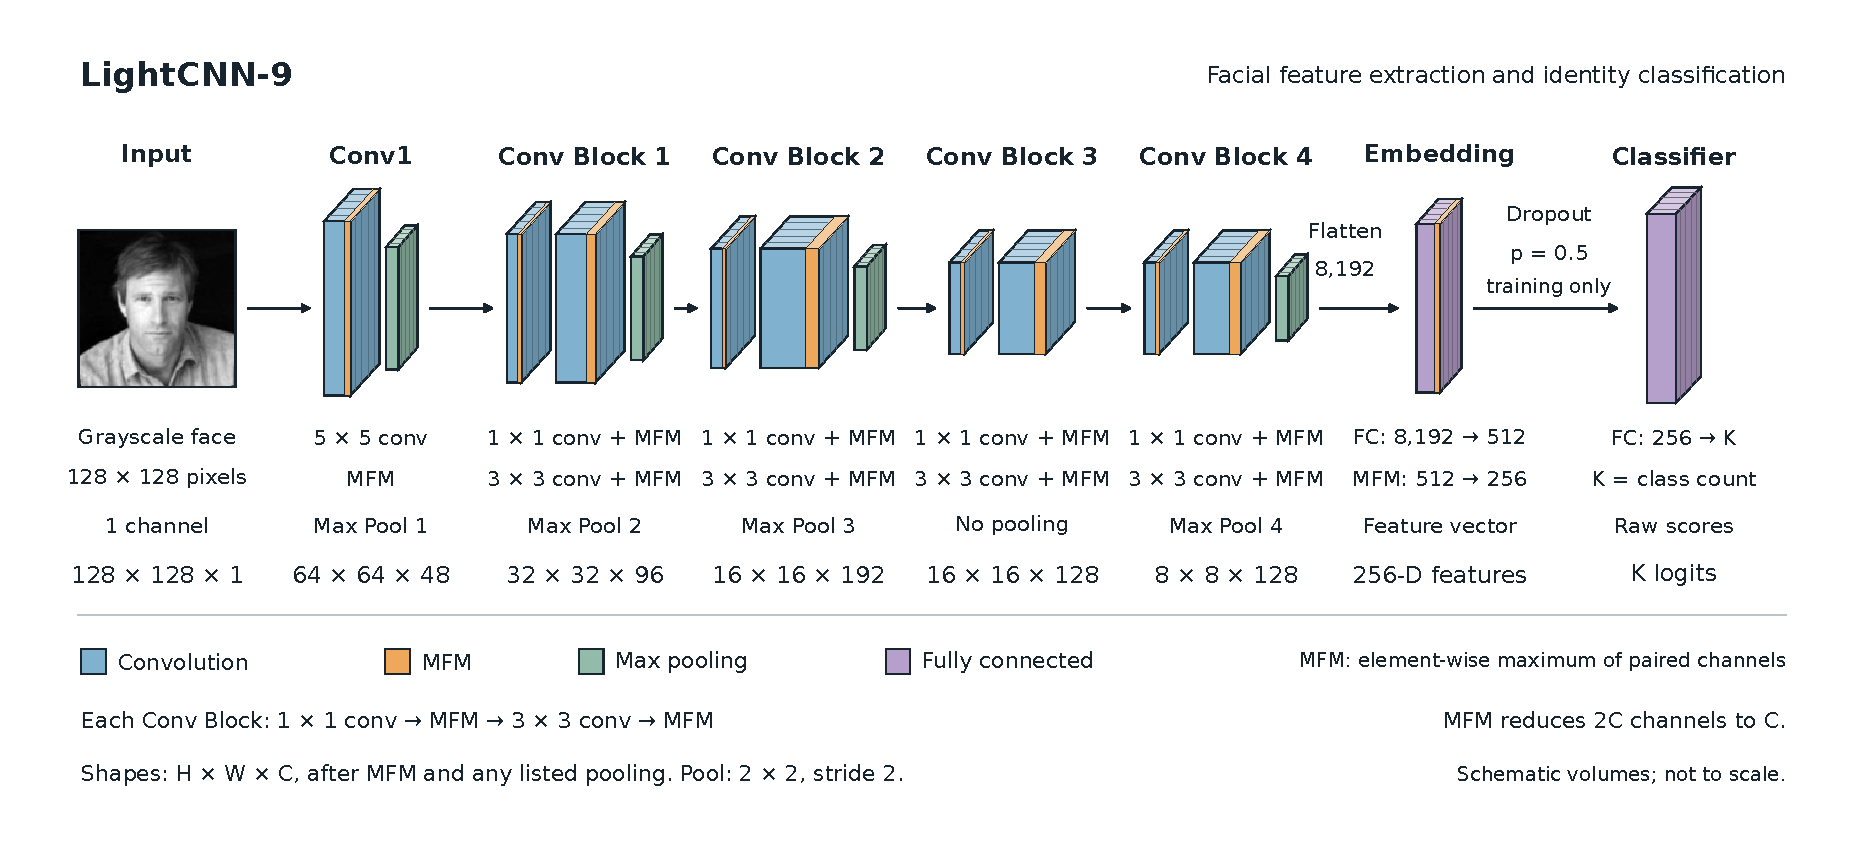
\includegraphics[width=\textwidth]{figures/lightcnn9_publication.pdf}
    \caption{Architecture of LightCNN-9 showing the convolution blocks, MFM operations, pooling layers, 256-dimensional embedding, and identity classifier.}
    \label{fig:lightcnn9_architecture}
\end{figure*}

According to the original paper, LightCNN-9 contains approximately 5.556 million parameters and requires approximately 1 GFLOP. It produces a 256-dimensional facial representation and requires approximately 67 ms for feature extraction on a single core of an Intel i7-4790 processor. The paper reports 98.80\% accuracy on LFW and 93.40\% accuracy on YTF under its stated evaluation protocols \cite{wu2018lightcnn}.

The smaller model size, low-dimensional representation, and use of grayscale images make LightCNN-9 a suitable candidate for real-time facial recognition. However, its fully connected layer requires a fixed input size, and the reported processing time depends on the hardware used by the original authors. The LFW result also represents face verification rather than the identity-classification task required by our final system. For our implementation, the final classifier can be replaced with a new classifier for the identities in our own dataset while retaining the earlier layers for facial feature extraction.


% ============================================================
% III. ARCHITECTURE 2
% ============================================================

\section{Architecture 2: FaceNet}

FaceNet is a unified system for face verification, recognition, and clustering, which builds upon the Siamese Neural Network (SNN) architecture. Each face is mapped onto the Euclidean space. The network is trained such that the embeddings of similar data points converge closer together within the feature space, while simultaneously pushing embeddings of dissimilar data points to drift further apart; meaning images of the same person are close together in the learned space and vice versa in the case of images of different people \cite{schroff2015facenet}.

It also uses a triplet loss function. To calculate triplet loss, we use images corresponding to the anchor, positive, and negative.

\begin{center}
    \centering
    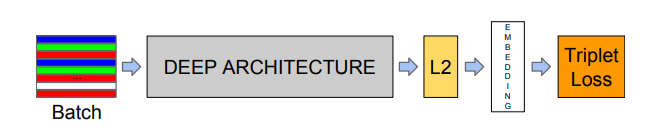
\includegraphics[width=\columnwidth]{figures/facenet_model_structure.png}
    \captionof{figure}{Model Structure of FaceNet}
    \label{fig:facenet_model_structure}
\end{center}

The network consists of an input layer, a deep CNN, followed by L2 normalization, which results in the face embedding. This is then followed by the triplet loss.

\textbf{Triplet Loss and Selection}

The loss function is defined using triplets of training points of the form (A, P, N).

A = anchor (reference image)\\
P = positive (if the image is of the same person as A)\\
N = negative (if the image is of a different person than A)

Triplet loss minimizes the distance between the anchor and the positive, while maximizing the distance between the anchor and the negative (see Figure~\ref{fig:facenet_triplet_loss}).

\begin{center}
    \centering
    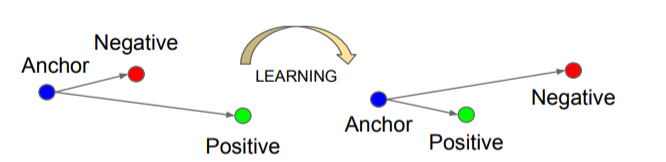
\includegraphics[width=\columnwidth]{figures/facenet_triplet_loss.png}
    \captionof{figure}{Triplet Loss}
    \label{fig:facenet_triplet_loss}
\end{center}

Triplet loss can be formalized as:

\begin{equation}
\begin{aligned}
L=\sum_i^N\big[&\left\|f(x_i^a)-f(x_i^p)\right\|_2^2 \\
&-\left\|f(x_i^a)-f(x_i^n)\right\|_2^2+\alpha\big]_+
\end{aligned}
\label{eq:facenet_triplet_loss}
\end{equation}

$\alpha$ here is defined as the margin that is enforced between positive and negative pairs.

Generating all possible triplets would result in multiple triplets that already satisfy the constraint. These triplets would not contribute to the training and would result in slower convergence. And thus it is important to select hard triplets which can therefore contribute to improving the model.

\textbf{Deep Convolution Networks}

FaceNet trains CNNs using Stochastic Gradient Descent (SGD) with standard backdrop and AdaGrad.

SDG is an optimization model that is used to optimize the loss function

\begin{center}
    \centering
    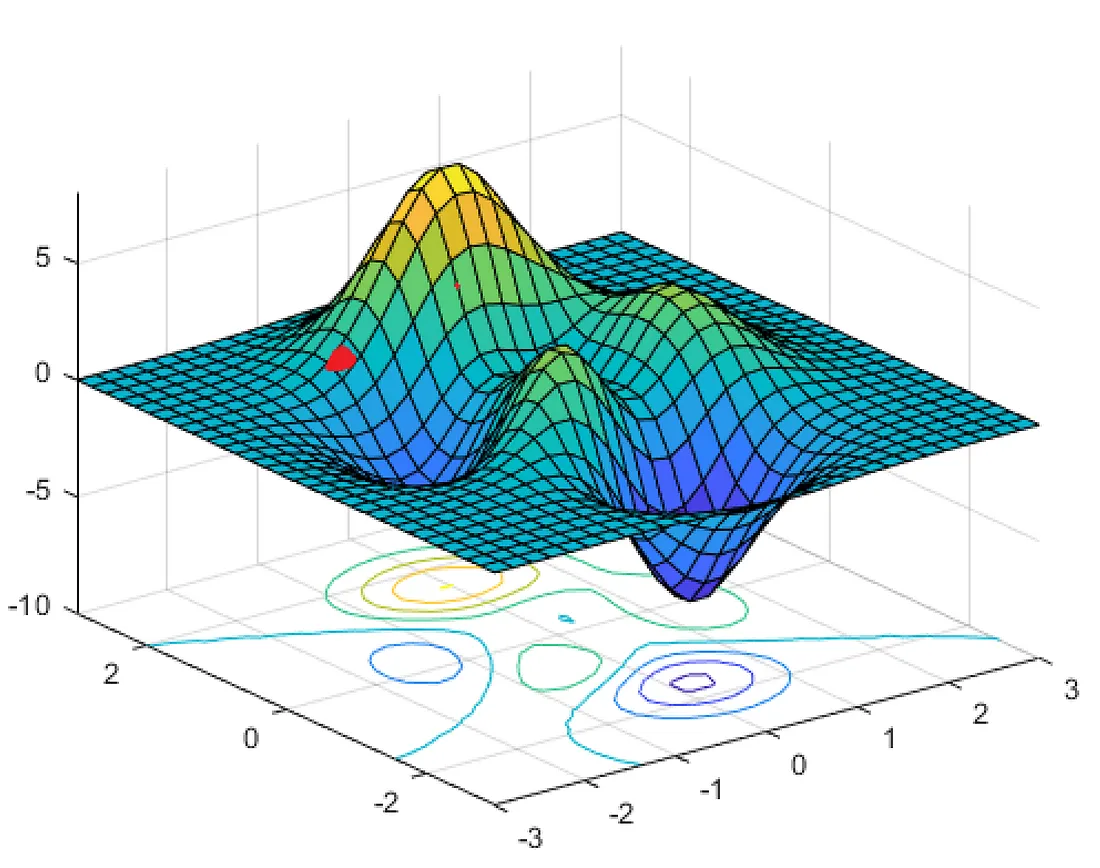
\includegraphics[width=\columnwidth]{figures/facenet_sdg.png}
    \captionof{figure}{SDG (Credit - \textit{datascience.stackexchange})}
    \label{fig:facenet_sdg}
\end{center}

The x-axis and y-axis represent the weights while the z-axis is the loss corresponding to those weights. The intuition behind SDG is to traverse the hill-like structure using a point in such a way that the global minima can be obtained.

In SGD, the gradient is a vector which indicates the direction of the steepest local increase. SGD then updates the parameter in the opposite direction to minimize the loss, using gradients estimated from randomly sampled training data.

While AdaGrad is utilized here to dynamically generate variable learning rates, as fixed learning rates are impractical in deep learning.

\textbf{ReLU (Rectified Linear Unit)}

ReLU is a non-linear activation function. Without non-linear activation functions, even multiple layers of convolution would collapse into a single linear transformation. Also, without activation functions, complex and intricate patterns cannot be learned effectively, as the decision boundary would remain linear.

ReLU is a widely used alternative to traditional activation functions such as sigmoid and tanh. This activation function helps mitigate the vanishing gradient problem, as its gradient remains constant for positive inputs.

\begin{center}
    \centering
    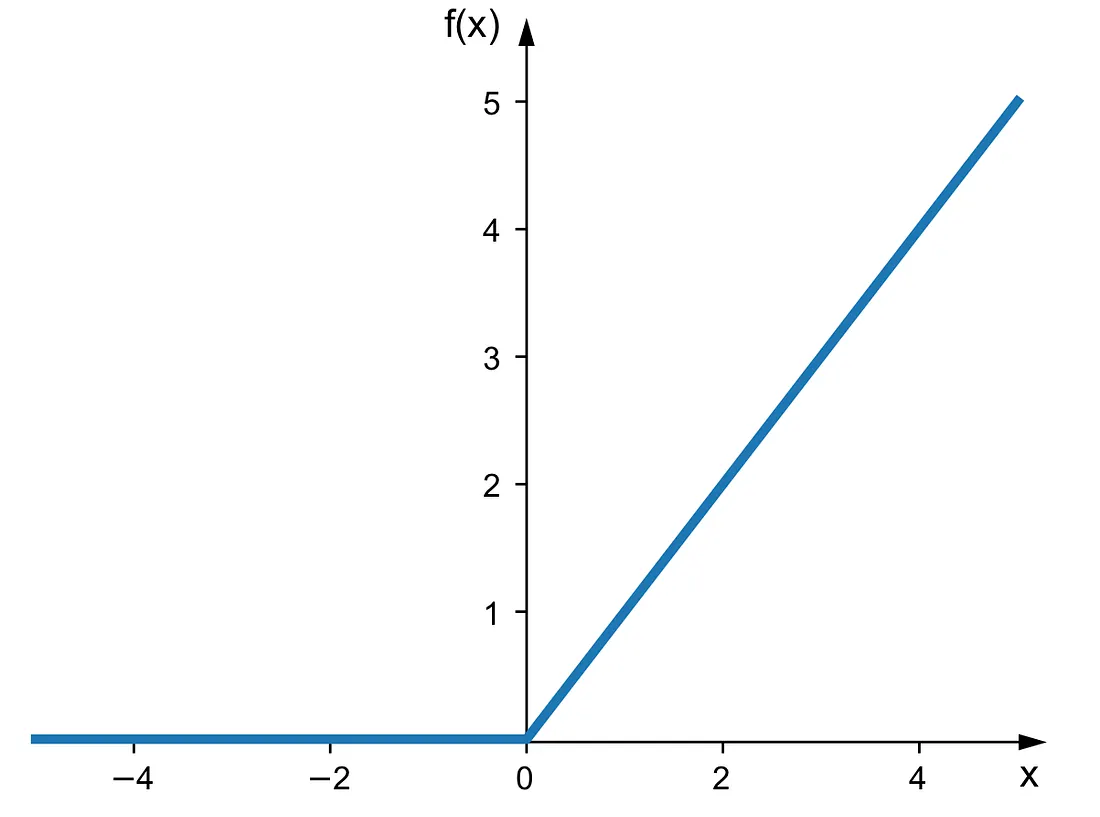
\includegraphics[width=0.88\columnwidth]{figures/facenet_relu.png}
    \captionof{figure}{ReLU activation function}
    \label{fig:facenet_relu}
\end{center}

\textbf{CNN Architectures}

The two types of CNN architectures used in FaceNet are Zeiler \& Fergus architecture and Inception Model.

Zeiler \& Fergus architecture - This architecture introduced a novel visualization technique that gives insight into the function of intermediate layers and the operation of classifiers in a CNN.

\begin{center}
    \centering
    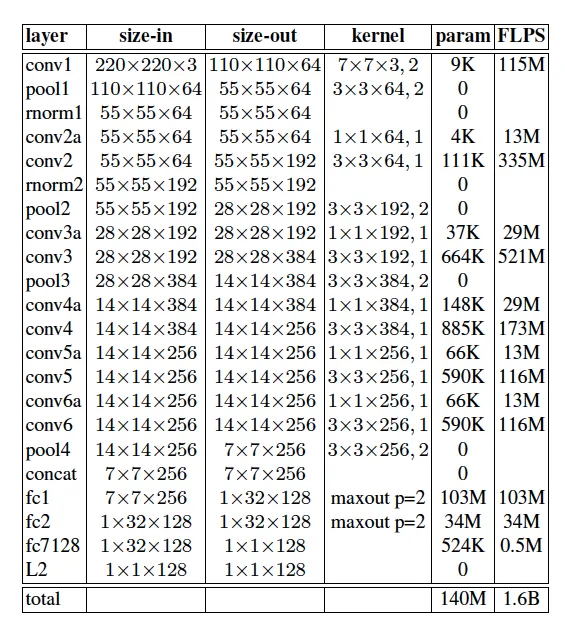
\includegraphics[width=0.92\columnwidth]{figures/facenet_zeiler_fergus.png}
    \captionof{figure}{Zeiler \& Fergus architecture used in FaceNet}
    \label{fig:facenet_zeiler_fergus}
\end{center}

Inception Model - The architecture was first introduced by the researchers at Google to curb the exorbitant resource requirement of deep neural networks. The Inception architecture combines 1x1, 3x3 and 5x5 Convulation filters in parallel and extract the features from the input image at different scales. The output of each filter is concatenated and passed to the next layer. This process is then repeated. This approach helps capture the local and global features while also minimizing the number of parameters required.

\begin{center}
    \centering
    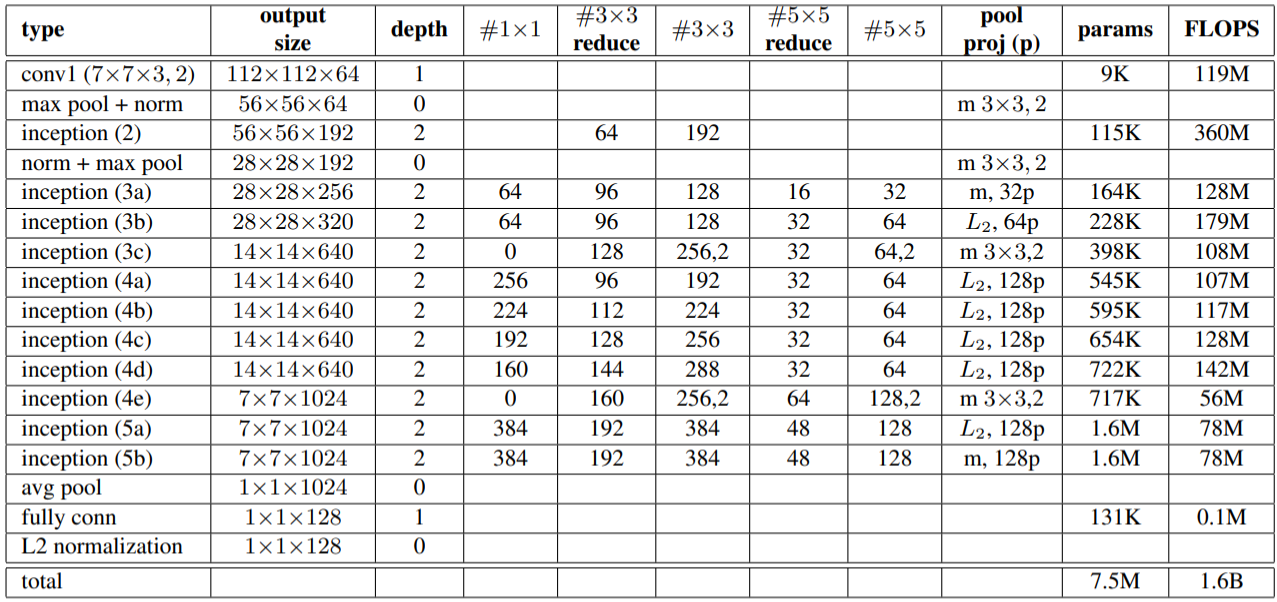
\includegraphics[width=\columnwidth]{figures/facenet_inception.png}
    \captionof{figure}{Inception Model used in FaceNet}
    \label{fig:facenet_inception}
\end{center}

\textbf{Performance of FaceNet Model on LFW}

The model is evaluated on two modes:

Fixed center crop of the LFW provided thumbnail.

A face detector is run on the LFW thumbnails. If it fails to align the images, the LFW alignment is used.

FaceNet achieves a classification accuracy of \textbf{98.87\% $\pm$ 0.15} when using the fixed center crop and \textbf{99.65\% $\pm$ 0.09} standard error of the mean when using the extra face alignment.

\begin{center}
    \centering
    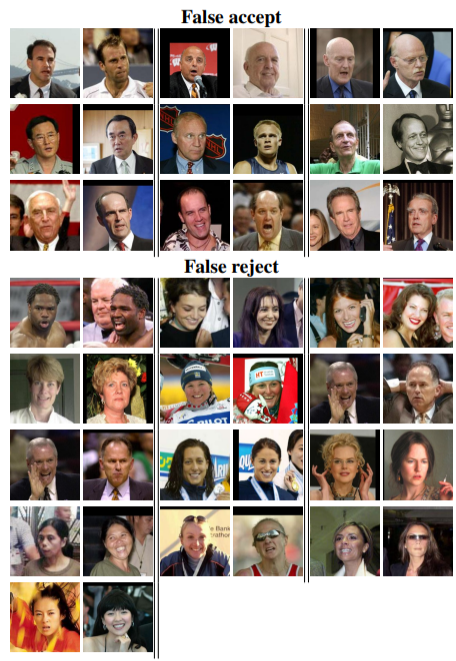
\includegraphics[width=0.88\columnwidth]{figures/facenet_lfw_errors.png}
    \captionof{figure}{LFW errors. This shows all pairs of images that were incorrectly classified on LFW}
    \label{fig:facenet_lfw_errors}
\end{center}

\textbf{Conclusion}

With an accuracy of \textbf{99.65\% $\pm$ 0.09} on the LFW dataset, FaceNet demonstrates the effectiveness of embedding-based approaches in face recognition.


% ============================================================
% IV. ARCHITECTURE 3
% ============================================================

\section{Architecture 3: Name}

\textit{[Write the analysis of Architecture 3 here.]}


% ============================================================
% V. ARCHITECTURE 4
% ============================================================

\section{Architecture 4: Name}

\textit{[Write the analysis of Architecture 4 here.]}


% ============================================================
% VI. ANALYSIS AND DISCUSSION
% ============================================================

\section{Analysis and Discussion}

The four architectures will be compared using the results reported in their original research papers. LFW is selected as the primary dataset because it is widely used for evaluating facial recognition models. YTF is selected as the second dataset because it evaluates recognition from video frames containing changes in pose, expression, lighting, and image quality. A result will only be treated as a direct comparison when the models use the same dataset, evaluation protocol, and performance metric. Results obtained using different protocols will be discussed separately. Along with recognition performance, the comparison will consider the number of parameters, embedding dimension, inference time, and the hardware used for testing. Table~\ref{tab:architecture_comparison} provides the common structure for recording these results. The remaining values will be added after the other architectures have been studied.

\begin{table*}[t]
    \centering
    \caption{Preliminary comparison of the four facial recognition architectures using results reported in their original papers.}
    \label{tab:architecture_comparison}
    \begin{tabular}{lccccc}
        \toprule
        \textbf{Architecture} & \textbf{LFW Acc. (\%)} & \textbf{YTF Acc. (\%)} & \textbf{Parameters} & \textbf{Embedding} & \textbf{Inference time} \\
        \midrule
        LightCNN-9 & 98.80 & 93.40 & 5.556M & 256-D & 67 ms$^{a}$ \\
        FaceNet & 99.65$^{b}$ & 95.12 & 7.5M$^{c}$ & 128-D & --$^{d}$ \\
        Architecture 3 & -- & -- & -- & -- & -- \\
        Architecture 4 & -- & -- & -- & -- & -- \\
        \bottomrule
    \end{tabular}

    \vspace{2pt}
    \begin{minipage}{0.96\textwidth}
        \footnotesize\textit{$^{a}$Reported for feature extraction using one core of an Intel i7-4790 processor. $^{b}$The supplied FaceNet document reports 99.65\% $\pm$ 0.09 using extra face alignment. $^{c}$The Inception model table reports 7.5M parameters and 1.6B FLOPS. $^{d}$Inference time and tested hardware are not reported. Accuracy values should only be compared directly when the evaluation protocols are equivalent.}
    \end{minipage}
\end{table*}


% ============================================================
% VII. CONCLUSION
% Required: approximately 100 words
% ============================================================

\section{Conclusion}

\textit{[Write the approximately 100 word conclusion here.]}


% ============================================================
% REFERENCES
% IEEE FORMAT
% ============================================================

\begin{thebibliography}{99}

% Example:
%
% \bibitem{example}
% A. Author, B. Author, and C. Author,
% ``Title of paper,''
% \textit{Journal or Conference Name},
% vol. X, no. X, pp. XX--XX, Year.

\bibitem{wu2018lightcnn}
X. Wu, R. He, Z. Sun, and T. Tan,
``A light CNN for deep face representation with noisy labels,''
\textit{IEEE Transactions on Information Forensics and Security},
vol. 13, no. 11, pp. 2884--2896, 2018.

\bibitem{schroff2015facenet}
F. Schroff, D. Kalenichenko, and J. Philbin,
``FaceNet: A unified embedding for face recognition and clustering,''
in \textit{Proceedings of the IEEE Conference on Computer Vision and Pattern Recognition},
pp. 815--823, 2015.

\end{thebibliography}


\end{document}
